\begin{figure} \centering 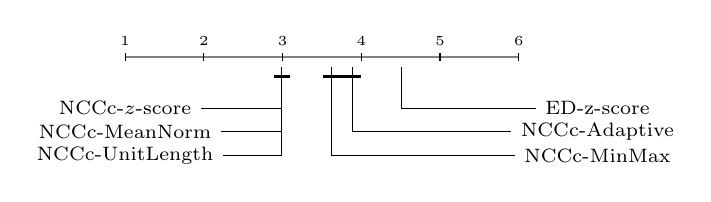
\begin{tikzpicture}[xscale=2]
\draw[gray, thick](00.5000, 0) -- (03.0000, 0);
\foreach \x in {00.5000,01.0000,01.5000,02.0000,02.5000,03.0000}\draw (\x cm,1.5pt) -- (\x cm, -1.5pt);
\node (Label) at (00.5000,0.2) {\tiny{1}};
\node (Label) at (01.0000,0.2) {\tiny{2}};
\node (Label) at (01.5000,0.2) {\tiny{3}};
\node (Label) at (02.0000,0.2) {\tiny{4}};
\node (Label) at (02.5000,0.2) {\tiny{5}};
\node (Label) at (03.0000,0.2) {\tiny{6}};
\draw[decorate,decoration={amplitude=.4mm,segment length=1.5mm,post length=0mm}, very thick, color = black](01.4460,-00.2500) -- ( 01.5460,-00.2500);
\draw[decorate,decoration={amplitude=.4mm,segment length=1.5mm,post length=0mm}, very thick, color = black](01.7585,-00.2500) -- ( 01.9955,-00.2500);
\node (Point) at (01.4960, 0){};  \node (Label) at (0.5,-00.6500){\scriptsize{NCCc-$z$-score}}; \draw (Point) |- (Label);
\node (Point) at (01.4960, 0){};  \node (Label) at (0.5,-00.9500){\scriptsize{NCCc-MeanNorm}}; \draw (Point) |- (Label);
\node (Point) at (01.4960, 0){};  \node (Label) at (0.5,-01.2500){\scriptsize{NCCc-UnitLength}}; \draw (Point) |- (Label);
\node (Point) at (02.2580, 0){};  \node (Label) at (3.5,-00.6500){\scriptsize{ED-z-score}}; \draw (Point) |- (Label);
\node (Point) at (01.9455, 0){};  \node (Label) at (3.5,-00.9500){\scriptsize{NCCc-Adaptive}}; \draw (Point) |- (Label);
\node (Point) at (01.8085, 0){};  \node (Label) at (3.5,-01.2500){\scriptsize{NCCc-MinMax}}; \draw (Point) |- (Label);
\end{tikzpicture}
\vspace{-0.3cm}
\caption{Ranking of different normalization methods for $NCC_{c}$ based on the average of their ranks across datasets, using ED with $z$-score as the baseline method.}
\label{fig:sliding2}
\vspace{-0.2cm}
\end{figure}




\newline \textbf{Modifications in datasets:} The bottleneck in all distance-based classifiers, including our version, is the computation of the dissimilarity matrixes $W$ and $E$. Specifically, for the original version of the 128 datasets, we need to invoke about $257$ million times a distance measure to compute $E$ and, if parameter turning is required, we need to invoke the distance measure an additional $92$ million times to compute $W$, for each parameter, often resulting in close to $3$ billion invocations for a single distance measure. Overall, we estimate that we require to perform several trillions of such invocations to compute about $58,000$ test accuracy numbers for the $63$ distance measures over the $128$ datasets, including the combinations with the $8$ normalization methods. 

%\vspace*{-0.1cm}
\begin{figure}
	\vspace*{-0.3cm}
	\centering
	\subfloat[Reduced length]{{\label{fig:lengthdownsampling}}{\includegraphics[height=4.1cm,width=4.1cm]{figures/1NNEDOriginalvsModifiedDownsample-crop.pdf}
	}}%
	%\qquad
	\subfloat[Reduced size]{{\label{fig:sizedownsampling}}{\includegraphics[height=4.1cm,width=4.1cm]{figures/1NNEDOriginalvsModifiedStratified-crop.pdf}
	}} \vspace*{-0.2cm}
	\caption{Comparison of 1-NN+ED classifiers over the original datasets against the modified datasets with reduced (a) time-series lengths and (b) training and test sets sizes. Each circle represents a dataset and circles above the diagonal  indicate original datasets that outperform modified datasets.}%
    %\vspace*{-0.2cm}
	\label{fig:modifieddatasets}%
\end{figure}

Considering that several of the distance measures we study are very computationally expensive, especially with the increasing length of time series, we perform two additional preprocessing steps to enable this massive experimentation. First, for datasets with training or test sets containing more than $1000$ time series, we perform a stratified sampling to reduce the time series in these sets close to $1000$ while preserving the class distribution of the datasets. Second, for datasets with time series of length more than $1000$, we perform a downsampling to reduce the length to $500$. These two steps have reduced by $10x$ the storage requirements and by $20x$ the computational requirements, enabling us to perform the study in a period of one month using the resources described next. Importantly, these two steps result in negligible differences in the accuracy of the datasets. 

Specifically, Figure \ref{fig:modifieddatasets} compares 1-NN accuracy numbers obtained with ED (1-NN+ED) over the original $128$ datasets and their modified versions with reduced (i) time-series lengths (Figure \ref{fig:lengthdownsampling}) and (ii) training and test sets sizes (Figure \ref{fig:sizedownsampling}). Each circle represents a dataset, and the coordinates indicate the accuracy of the dataset for the methods in the $x$-axis and $y$-axis. Therefore, circles on the diagonal indicate no difference in accuracy, and circles above the diagonal indicate that the method in the $y$-axis outperforms the method in $x$-axis. We observe that downsampling long time series significantly affects only three datasets (Figure \ref{fig:lengthdownsampling}) whereas downsampling large training and test sizes significantly affects only $10$ datasets, overall less than $10\%$ of all datasets. Importantly, for fairness, we evaluate {\em all} measures over all new modified dataset versions to ensure the exact same settings.

\begin{table}[]
\footnotesize
\centering
%%\resizebox{\textwidth}{!}{%
\begin{tabular}{|c|c|c|c|c|c|c|c|c|c|}
\hline
\multirow{2}{*}{\textbf{Dataset categories}} & \multicolumn{9}{c|}{\textbf{Distance Measures}} \\ \cline{2-10} 
 & \textbf{1} & \textbf{2} & \textbf{3} & \textbf{4} & \textbf{5} & \textbf{6} & \textbf{7} & \textbf{8} & \textbf{9} \\ \hline \hline
\textbf{IMAGE (32)} & 2 & 6 & \textbf{8} & 5 & 5 & 1 & 1 & 7 & 3 \\ \hline
\textbf{MOTION (25)} & 2 & 1 & \textbf{8} & 5 & 2 & 1 & 3 & 8 & 0 \\ \hline
\textbf{SENSOR (22)} & 4 & 4 & \textbf{5} & 3 & 4 & 1 & 2 & 4 & \textbf{5} \\ \hline
\textbf{SPECTRO (12)} & \textbf{4} & 3 & 3 & 2 & 0 & 1 & 2 & 2 & \textbf{4} \\ \hline
\textbf{DEVICE (10)} & 1 & 1 & 1 & 2 & 2 & 0 & 0 & 1 & \textbf{3} \\ \hline
\textbf{SIMULATED (9)} & 1 & 0 & 0 & \textbf{4} & 0 & 0 & 2 & 1 & 2 \\ \hline
\textbf{ECG (7)} & 1 & 3 & 0 & 0 & 0 & 0 & 0 & 0 & \textbf{4} \\ \hline
\textbf{HEMODYNAMIC (3)} & 0 & 1 & 1 & 0 & 1 & 0 & 1 & 1 & 0 \\ \hline
\textbf{EOG (2)} & 0 & 0 & 0 & \textbf{2} & 0 & 0 & 0 & 0 & 0 \\ \hline
\textbf{EPG (2)} & 0 & 0 & 1 & 1 & 0 & 0 & 0 & 1 & 0 \\ \hline
\textbf{TRAFFIC (2)} & 0 & 1 & 0 & 0 & 0 & 0 & 0 & 1 & 0 \\ \hline
\textbf{SOUND (1)} & 0 & 0 & 0 & 0 & 0 & 0 & 0 & \textbf{1} & 0 \\ \hline
\textbf{OTHER (1)} & 1 & 1 & 1 & 1 & 1 & 1 & 1 & 1 & 1 \\ \hline \hline
\textbf{\# Best} & \textbf{16} & \textbf{21} & \textbf{28} & \textbf{25} & \textbf{15} & \textbf{5} & \textbf{12} & \textbf{28} & \textbf{22} \\ \hline 
\end{tabular}%
%%}
\caption{Best performing distance measures split by dataset type. 1 = Lorentzian with MeanNorm, 2 = $NCC_c$, 3 = MSM, 4 = DTW, 5 = EDR, 6 = LCSS, 7 = Swale, 8 = TWE, 9 = ERP.}
\label{tab:overall_ranking}
\end{table}